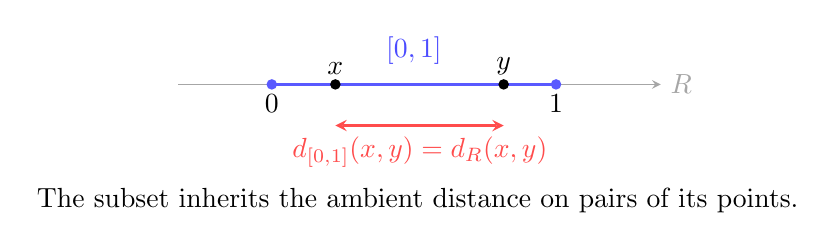
\begin{tikzpicture}[scale=0.95,>=stealth]
  \draw[->,gray!70] (-0.25,0) -- (6.2,0) node[right] {\(\mathbb{R}\)};
  \draw[blue!65,very thick] (1.0,0) -- (4.8,0);
  \fill[blue!65] (1.0,0) circle (2pt);
  \fill[blue!65] (4.8,0) circle (2pt);
  \node[below] at (1.0,0) {\(0\)};
  \node[below] at (4.8,0) {\(1\)};
  \node[blue!70] at (2.9,0.45) {\([0,1]\)};

  \fill[black] (1.85,0) circle (2pt);
  \fill[black] (4.1,0) circle (2pt);
  \node[above] at (1.85,0) {\(x\)};
  \node[above] at (4.1,0) {\(y\)};
  \draw[<->,red!70,thick] (1.85,-0.55) -- (4.1,-0.55);
  \node[red!70] at (2.98,-0.9) {\(d_{[0,1]}(x,y)=d_{\mathbb{R}}(x,y)\)};

  \node[align=center] at (2.95,-1.55)
    {The subset inherits the ambient distance on pairs of its points.};
\end{tikzpicture}
